\documentclass[12pt, letterpaper]{article}
\usepackage[utf8]{inputenc}
\usepackage{graphicx}

\title{User Manual for LeetCode}
\author{Chaolei CAI}

\begin{document}


\begin{titlepage}
    \maketitle
\end{titlepage}

\tableofcontents
\section{Introduction}
This is an user manual to introduce the website LeetCode.com, which an platform that allow you solve differents problems in computer science field. The application is mainly free, there are few content that you need to pay to acces(e.g: new interview question for GAFA). However in my personal user experience, I never felt the need to acces to those contents. The platform aleady provide for free over a thousand of interview question with 3 difficulties (easy, medium and hard)



\section{Installation guide}
To begin with, you will need to create an account in order to acces the platform. It is possible to log in with you social network account such like facebook, google or github.

\begin{figure}
    
\includegraphics[width=\linewidth]{img/L1.png}
    \caption{Welcome page}
    \label{fig:L1}
    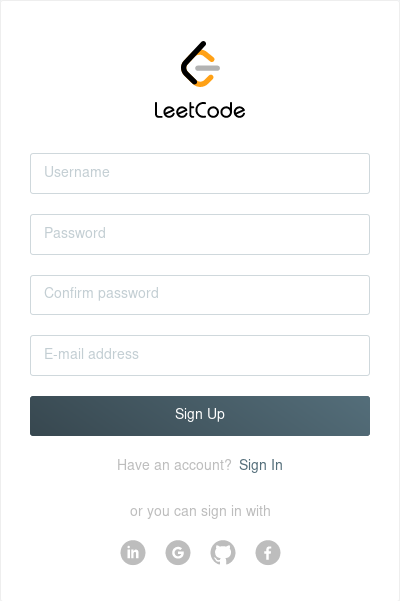
\includegraphics[width=\linewidth]{img/L2.png}
    \caption{Sign up page}
    \label{fig:L1}
\end{figure}

\section{Get started}
Once you have logged in, you can see this panel at the top.\\

\includegraphics[width=\linewidth]{img/L3.png}
\subsection{Explore}
If you have no specific idea of what you want to improve, try this section.\\
Explore section allow you to explore different collection of problem classed by theme.\\
It could be very precise target like Apple/Amazon/Google interview questions or very basic computer science field algorithm or data structure. \\

\subsection{Problems}
Scroll down your mouse and you will see this interface.\\
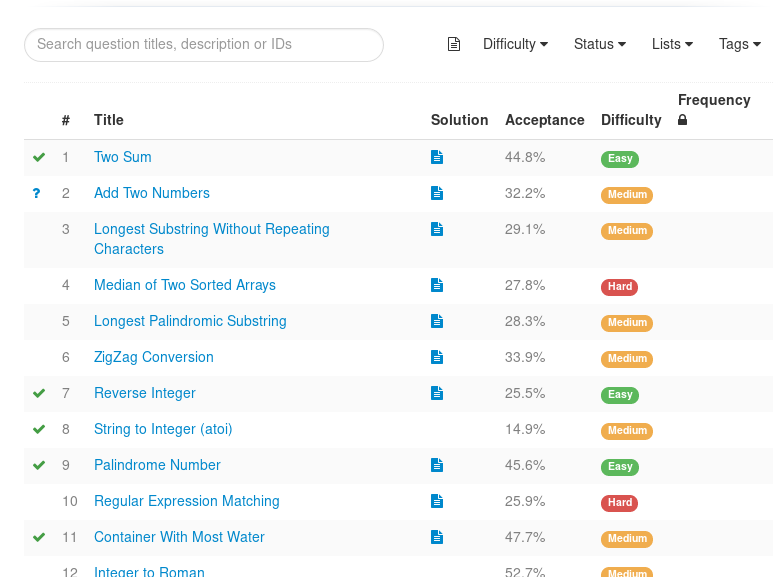
\includegraphics[width=\linewidth]{img/L5.png}
Remember the thousand of problem that I've promessed? There you got.\\
You can follow the question order or start with the easiest or the hardest.\\
In my personal experience, most of time I need to spend 30min for a easy question,
1hour for a medium. I've never solved hard level question because in my personal opinion it's not worthy to spend that much of time, at that level of difficultie, you have to solve it with a lot of constraint such like time complexity or space complexity (If you don't know what it is, it force your program to run over in a certain time and only use a limited memory space).\\
I can't denie the fact of how it is interesting to program with limited ressources, however I am using LeetCode for academic use rather to proof my programming skill to my future employer.

\subsection{Mock}
Mock section is a kind of real time simulation to an job interview, you will be given a limited time to solve one or more question. To be honest, I never used this section because you have to pay to acces specific company's question base. If you are a "free" user like me, you can only draw question randomly.

\subsection{contest}
Let's move on to contest section, if you want to proof your programming skill, this section is made for you.
Each week, the website organize an contest that everyone can participate. \\
The rule is simple, you will be given a limited time to solve a list of question.\\
The goal is to be the fastest, to add some difficultie, each wrong answer will be associated with a short time penalty.\\
The price is what we call LeetCode point, what is its purpose? Well, you can exchange it for goodies like pen or t-shirt...

\subsection{Article}
In this section, you can acces (well it's not going to be free) question's official solution.
I will explain you in further

\subsection{Profile}
Click on your profile picture to access quick profile bar.\\
From there, you can acces to differents settings and functionality like progress bar or your favorite.\\
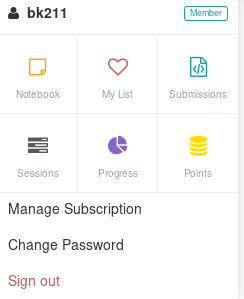
\includegraphics{img/L4.png}\\
Click on your ID to access your personal profile page.\\
You can see your last submission, your daily activities or the linking to others social network page (e.g: Linkedin, Google, Github and Facebook).
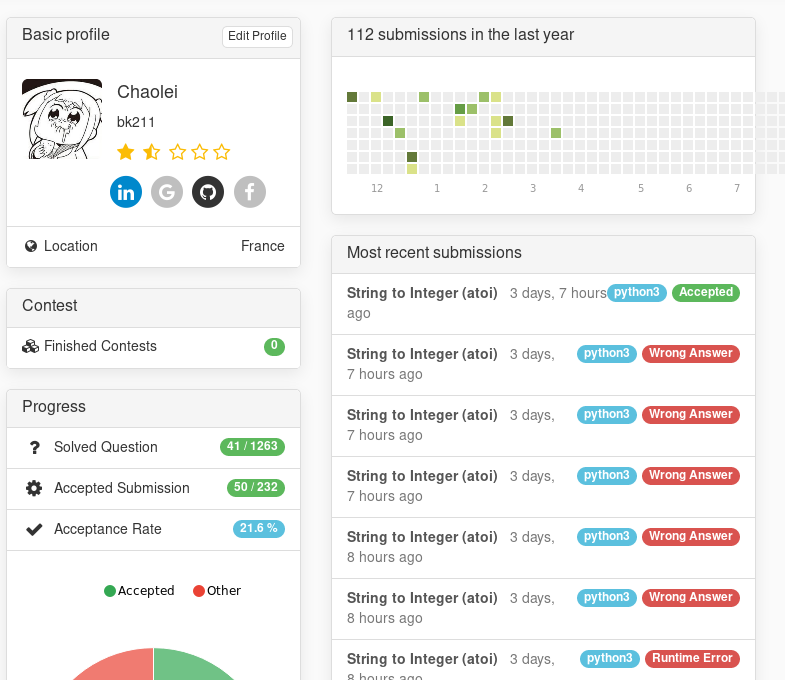
\includegraphics[width=\linewidth]{img/L6.png}

\section{The Playground}
Click an problem to start it, you will access to the "playground".\\
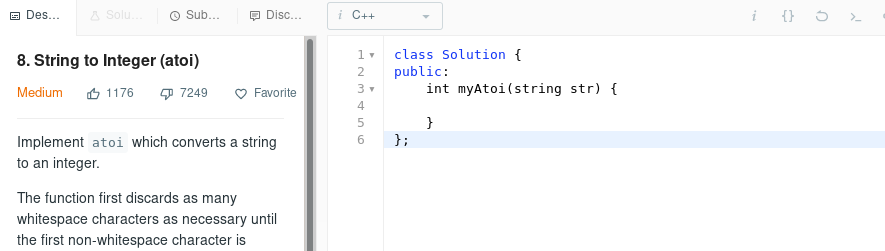
\includegraphics[width=\linewidth]{img/L7.png}\\

The playground is divided by 2 colums, at the left side, you can read the problem, most of them have few example to illutrate. Finally, at your right side, you have the coding environnement, one of the key feature of LeetCode is that you can run it in an browser, there are nothing to install nor any environment to set up, you are totally free to use any* language to resolve the problem.\\
*LeetCode support most part of currently popular programming language (C++,Python2/3,C, Java, Javascript etc.)

Once your have done coding or you want to launch a test, all you have to do is click the "run code" at the right bottom, your code with be tested with the test-case next to you.\\

\includegraphics{img/L8.png}\\

This process can be a little bit long, so most of time I'm used to test my code on my local machine with one specific test case. Just to check if my solution can handle this unique test-case.
At the end, if you are sure with solution, you can click the "submit" button, your code with be tested with all test-case.\\
Then finally if you pass all test-case, your solution is accepted and you can see the speed of your solution. Also, your program's performance is compared to the others.\\
In my personal opinion if you are under 20\% you can consider it as very fast, I do not advice you to target the 5\% since most of them are made of low level optimisation such like bitwise operation or syntaxique sugar for a specific programming language.\\
That been said, I highly suggest to look at the others solutions, it is also an improvement to be able to read others people's code. You can ask yourself questions like why he did it that way? What is different with my solution? Why it is faster or slower than mine etc.\\
beetween 20 and 70\% I consider it as an good score, if you are over 70\%, that not too bad, you provided an succesful solution, there are probably some optimisation to perform.\\


\section{System requirement}
All you need is a decent browser to have a decent user experience from the website.\\
I advice you to use popular browser like chrome, safari, firefox.\\
(Some say that the last microsoft Edge is pretty "ok", but due to his very bad reputation from the past, let's ignore it).
\section{Troubleshooting}
For any question that I've not treated, please contact me by email
\section{Terms and conditions}
I do not have any relationship with LeetCode and I didn't received any salary or royaltie to promote LeetCode, thus I do not engage any resposability for the conscequences of your usage of LeetCode platform.


\end{document}
